\documentclass[a4paper,12pt]{article}
\usepackage[english]{babel}
\usepackage[utf8]{inputenc}
\usepackage{amsmath}
\usepackage{amsthm}
\usepackage{amsfonts}
\usepackage{amssymb}
\usepackage{graphicx}
\usepackage{hyperref}
\usepackage{enumitem}
\usepackage{float}
\usepackage{booktabs}
\usepackage{CJKutf8}
\usepackage[colorinlistoftodos]{todonotes}
\usepackage[left=1.50cm, right=1.50cm, top=1.20cm]{geometry}
\linespread{1.5}

\title{LeetCode 400---599}
\begin{document}
	\maketitle
\section{400-409}
\subsection{402 Remove K digits}
Given a non-negative integer num represented as a string, remove \textit{\textbf{k}} digits from the number so that the new number is the smallest possible.
\par
\vspace{0.5em}
\noindent
\textbf{\large{Note:}}
\begin{CJK*}{UTF8}{gbsn}
\begin{itemize}
\item 如果用贪心法,即每次从头开始找递减序列,然后删除递减序列的第一个字符,会超时
\item 快速的方法是: 从头开始遍历\textbf{num},将第一个字符放入结果中,然后如果继续,如果当前字符比结果的尾数要大,弹出尾部数字,直至到第一个在result的数字比这个数小。然后重复
\item 最后需要处理头部为0的情况
\item 另外,如果生成的结果数组长度大于原有长度和\textit{\textbf{k}}的差,就要重新\textit{resize}
\end{itemize}
\clearpage
\end{CJK*}

\subsection{403 -- Frog Jump}
\begin{figure}[H]
	\begin{center}
		\includegraphics[width=15cm]{403.png}
	\end{center}
\end{figure}
\textbf{\large{Note:}}
\begin{CJK*}{UTF8}{gbsn}
	\begin{itemize}
		\item 这个题目其实可以构造出一个树状结构,然后进行深度遍历
		\item 从第一个石头开始,第一个石头只有一个\textit{jump}值就是\textbf{1},所以从第一个石头往前面跳的$\text{step} = 1$ 或者 2,($\text{step}=0$没有意义)根据后面石头和这块石头的间隔以及可能的\textbf{step},可以得到可以跳到的下一块石头的位置。以题目给的例子为例,我们可以得出如下的树状图(图中每个节点用``[石头位置,跳到该位置所用的jump]''来表示).其中绿色的表示可以到达的石头,红色表示到不了的石头
		\begin{figure}[H]
			\begin{center}
				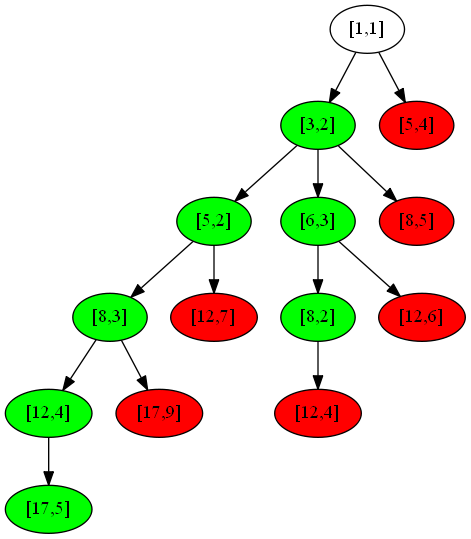
\includegraphics[width=15cm]{403_Example.png}
			\end{center}
		\end{figure}
		以节点[3,2]为例,从其下一个石头位置开始遍历,其下一个石头位置为5, $5-3=2$,所以可以跳到5, 再下一个石头位置为6, $6-3=3=2+1$, 因此也能跳到6, 接着是位置8的石头,$8-3=5>2+1$,所以这个位置不能到达,遍历停止。
		\item 遍历这个树状图,如果用递归法,那么递归函数参数包括,当前位置, 跳到当前位置所用的\textit{jump}和以及用于记录位置和\textit{jump}是否能到达的\textit{hashmap}。
		\item 在函数中,如果按照位置和\textit{jump},\textit{hashmap}能找到,则直接返回,否则,从该位置的下一个位置开始遍历,直至到达到不了的位置(即两个石头的间隔比JUMP+1还大),然后从可以到达的石头位置开始递归调用函数。
		\item 递归的终止条件还包括位置已经到达数组的末尾。
	\end{itemize}
	\clearpage
\end{CJK*}

\subsection{404 -- Sum of Left Leaves}
\begin{figure}[H]
	\begin{center}
		\includegraphics[width=18cm]{404.png}
	\end{center}
\end{figure}
\textbf{\large{Note:}}
\begin{itemize}
	\item For each node, check if it has left child and its left child is leaf. If it is, add the value.
	\item If the node has left child but is not leaf, recursive on this node. and then recursive on the node's right child.
\end{itemize}

\subsection{405 -- Convert a Number to Hexadecimal}
\begin{figure}[H]
	\begin{center}
		\includegraphics[width=18cm]{405.png}
	\end{center}
\end{figure}
\textbf{\large{Note:}}
\begin{itemize}
	\item Basic idea: Right shift the number 4 bits, and then mask with 0xF. 
	\item To stop the shift, either the number is zero or the number has been right shifted 7 times. The latter is dealing with the case when number is $-1$. Without latter, the shift will continue forever.
\end{itemize}




\subsection{407 -- Trapping Rain Water II}
	\begin{figure}[H]
		\begin{center}
		\includegraphics[width=18cm]{407.png}
		\end{center}
	\end{figure}
	\textbf{\large{Note:}}
	\begin{CJK*}{UTF8}{gbsn}
	\begin{itemize}
		\item 从边界开始,用一个priority\textunderscore queue来保存扫描到的节点高度,最小的高度放在最上面。同时每个元素还包括当前节点的row和col.
		\item 同时,用一个同样大小的visited二维数组来记录当前节点是否访问过。
		\item 然后逐个从queue中弹出节点,对每一个弹出的节点,从这个节点的位置搜寻上下左右的相邻4个节点,如果这些节点在数组范围内并且没有被访问过,就把其加入到queue中,并记录其访问过。同时需要记录遇到最大的高度,因为水会填满低洼处。
		\item 如果遍历中遇到的节点的高度比当前的最大高度小,那么该节点可以接住雨水,其所能容纳的雨水量即为高度差。
	\end{itemize}
	\clearpage
	\end{CJK*}

\subsection{410 -- Split Array Largest Sum}
\textbf{\large{Note:}}
\begin{CJK*}{UTF8}{gbsn}
	\begin{itemize}
		\item 由于数组中都是非负整数,所以连续子数组的和可能出现的最大的值是从所有元素中的最大值(即这个子数组只包含这个最大值元素)以及所有元素之和(这是可能的连续数组和的最大值)。
		\item 然后就用二分查找寻找符合条件的最大值。即根据一个给定的最大值,然后在原数组中看有几个连续的子数组的和小于或者等于这个最大值。
		\item 比较trivial的点,在寻找原数组中有几个连续的子数组和小雨或者等于给定的最大值的时候, 如果起始的计数值为0, 那么扫描数组结束后需要加上1, 这是因为如果从某个位置开始一直到数组最后一个数肯定是小于给定的最大值的,否则早就在这个位置或者之前就遇到大于最大值了。
		\item 如果得到的小于等于给定最大值的连续子数组的个数不大于题目要求的$m$,则说明这个当前的最大值有点大了,这时候右边的边界减一。
		\item 否则,说明这个最大值有点小了,这时候左边界加1。一直到左边界大于或者等于有边界。然后返回左边界。
	\end{itemize}
\clearpage
\end{CJK*}

\subsection{413 -- Arithmetic Slices}
	\begin{figure}[H]
	\begin{center}
		\includegraphics[width=18cm]{413.png}
	\end{center}
\end{figure}
\textbf{\large{Note:}}
\vspace{1em}
\begin{CJK*}{UTF8}{gbsn}
	\begin{itemize}
		\item Similar to \textbf{Count Element with Maximum Appearances}. 使用两个计数器,一个是当前遇到的符合三个数等差的个数$C$,另外一个则是总数$TC$。
		\item 从第三个数开始,检查当前的三个数是否等差,如果是$C=C+1$,同时$TC=TC+C$。这是因为$TC$是所有的等差数列比如一个四个元素的等差数列,其中包含了三个三元素的等差数列。
		\item 如果当前三个数不等差,$C=0$。
		\item 最后的$TC$即为所求结果。
	\end{itemize}
\end{CJK*}
	
	\section{500--509}
	\section{510--519}
	\section{520--529}
	\section{530--539}
	\subsection{531	Lonely Pixel I}
	Given a picture consisting of black and white pixels, find the number of black lonely pixels. The picture is represented by a 2D char array consisting of \textbf{B} and \textbf{W}, which means black and white pixels respectively. A black lonely pixel is character \textbf{B} that located at a specific position where the same row and same column don't have any other black pixels.
	\par
	\vspace{0.5em}
	\noindent
	\textbf{\large{Note:}}
	\begin{CJK*}{UTF8}{gbsn}
		\begin{itemize}
			\item Scan whole matrix, 对每一个\textbf{B},用一个\textit{unordered\_set}来记录\textit{column}. 用一个\textit{unordered\_set}来记录\textit{row}
			\item Scan whole matrix again, 对每一个\textbf{B}, 看其\textit{row}和\textit{col}个数是否是1,如果是,计数值加1.
		\end{itemize}
		\clearpage\end{CJK*}
	
	\section{540--549}
	\section{550--559}
	\section{560--569}
	
	\subsection{562 Longest Line of Consecutive One in Matrix}
	Given a 0 and 1 matrix \textbf{M}, find the longest line of consecutive one in the matrix. The line could be horizontal, vertical, diagonal or anti-diagonal.
	\par
	\vspace{0.5em}
	\noindent
	\textbf{\large{Note:}}
	\begin{CJK*}{UTF8}{gbsn}
		\begin{enumerate}
			\item 用4个DP数组来记录4个方向上的到当前位置的连续1的长度
			\item 对每一个方向上的$DP$, 都有类似的关系,以水平方向为例. 如果当前位置的左边是$0$, 那么${DP_{H}[i][j-1]}=0$, 如果是$1$, 那么${DP_{H}[i][j-1]}=1$ 或者是以这个位置为结束的连续1长度个数。所以如果当前位置是$0$, 那么$DP_{H}[i][j]$仍然是$0$, 否则就是$DP_{H}[i][j] = DP_{H}[i][j-1]+1$
			\item 每次到一个位置,计算出四个DP数组,然后把最大值保存在结果中,直到完成全部元素扫描
		\end{enumerate}
		\clearpage\end{CJK*}
	
	\subsection{566 Reshape the Matrix}
	You're given a matrix represented by a two-dimensional array, and two positive integers \textit{r} and \textit{c} representing the row number and column number of the wanted reshaped matrix, respectively.
	\par
	The reshaped matrix need to be filled with all the elements of the original matrix in the same row-traversing order as they were.
	\par
	If the `\textbf{reshape}' operation with given parameters is possible and legal, output the new reshaped matrix; Otherwise, output the original matrix.
	\par
	\noindent
	\textbf{Note:}
	\begin{enumerate}[label={[\arabic*]}]
		\item new r = $\text{pos} \div \text{cols}_{\text{new}}$
		\item new c = $\text{pos} \% \text{cols}_{\text{new}}$
		\item The new reshaped matrix must have $r \times c = \text{r}_{\text{old}} \times \text{c}_{\text{old}}$ 
	\end{enumerate}
	
	
	
	
	\section{570--579}
	\subsection{573 Squirrel Simulation}
	Find the minimal distance for the squirrel to collect all the nuts and put them under the tree one by one. The squirrel can only take at most one nut at one time and can move in four directions - up, down, left and right, to the adjacent cell. The distance is represented by the number of moves.
	\vspace{0.5em}
	\noindent
	\textbf{\large{Note:}}
	\begin{enumerate}[label={[\arabic*]}]
		\item If the squirrel is in the position of the tree, the distance is fixed.
		\item If not, test each nut by subtracting the distance from the squirrel to the nut and then from the nut to the tree from the fixed distance in [1].
	\end{enumerate}
	
	\subsection{575. Distribute Candies}
	\begin{CJK*}{UTF8}{gbsn}
		非常简单的题, 给一个数组,长度是偶数,里面的数字代表糖果的种类。平均分给两个小孩,问其中一个小孩能拿到的最多的糖果种类个数。方法很简单,用一个unordered\_set记录种类的个数,如果种类个数小于一半数组长度,返回这个种类个数,因为这一半数组已经能包含所有的糖果种类了。 如果种类个数大于一般数组长度,每个种类拿一个,所以就是数组长度了。
		\clearpage\end{CJK*}
	
	\section{580--589}
	
	\subsection{589 --- N-ary Tree Preorder Traversal }
	Given an \textit{n}-ary tree, return the \textit{preorder} traversal of its nodes' values.
	\par
	\vspace{0.5em}
	\noindent
	\textbf{\large{Note:}}
	\par
	\vspace{0.5em}
	\noindent
	\begin{CJK*}{UTF8}{gbsn}
		如果用递归非常简单,如果用iterative方法,用一个stack进行辅助,最开始把root压入栈中。然后每次弹出的node,按照倒序的顺序把子节点压入栈中。
		\clearpage\end{CJK*}
	
	\section{590--600}
	\subsection{590 --- N-ary Tree Postorder Traversal}
	Given an \textit{n}-ary tree, return the \textit{postorder} traversal of its nodes' values.
	\par
	\vspace{0.5em}
	\noindent
	\textbf{\large{Note:}}
	\par
	\vspace{0.5em}
	\noindent
	\begin{CJK*}{UTF8}{gbsn}
		如果用递归非常简单,如果用iterative方法,用一个stack进行辅助,最开始把root压入栈中。然后每次弹出的node,按照一般顺序把子节点压入栈中。最后得到的结果数组要\textit{reverse}
		\clearpage\end{CJK*}
	
	\subsection{591 --- Tag Validator}
	Given a string representing a code snippet, you need to implement a tag validator to parse the code and return whether it is valid. A code snippet is valid if all the following rules hold:
	\begin{enumerate}
		\item The code must be wrapped in a \textbf{valid closed tag}. Otherwise, the code is invalid.
		\item A \textbf{closed tag} (not necessarily valid) has exactly the following format:
		\par
		\textless \texttt{TAG\textunderscore NAME}\textgreater \texttt{TAG\textunderscore CONTENT}\textless \texttt{/TAG\textunderscore NAME}\textgreater
		\item A valid \texttt{TAG\textunderscore NAME} only contain \textit{upper-case} letters, and has length in range [1,9]. Otherwise, the \texttt{TAG\textunderscore NAME} is invalid.
		\item A valid \texttt{TAG\textunderscore CONTENT} may contain other valid closed tags, cdata and any characters (see note1) EXCEPT unmatched \textless, unmatched start and end tag, and unmatched or closed tags with invalid \texttt{TAG\textunderscore NAME}. Otherwise, the \texttt{TAG\textunderscore CONTENT} is invalid.
		\item A start tag is unmatched if no end tag exists with the same \texttt{TAG\textunderscore NAME}, and vice versa. However, you also need to consider the issue of unbalanced when tags are nested.
		\item A \textless is unmatched if you cannot find a subsequent \textgreater. And when you find a \textless or \textless/, all the subsequent characters until the next \textgreater should be parsed as \texttt{TAG\textunderscore NAME} (not necessarily valid).
		\item The cdata has the following format : \textless![\texttt{CDATA}[\texttt{CDATA\textunderscore CONTENT}]]\textgreater. The range of \texttt{CDATA\textunderscore CONTENT} is defined as the characters between \textless ![\texttt{CDATA}[ and the first subsequent ]]\textgreater
		\item \texttt{CDATA\textunderscore CONTENT} may contain any characters. The function of cdata is to forbid the validator to parse \texttt{CDATA\textunderscore CONTENT}, so even it has some characters that can be parsed as tag (no matter valid or invalid), you should treat it as regular characters.
	\end{enumerate}
	\par
	\vspace{0.5em}
	\noindent
	\textbf{\large{Note:}}
	\par
	\vspace{0.5em}
	\noindent
	\begin{CJK*}{UTF8}{gbsn}
		\begin{enumerate}
			\item 用一个stack来保存当前遇到的start tag的匹配end tag.
			\item 每次遇到\textless/,表示碰到了end tag,这时候和stack 的top元素进行比较。如果不相等,表示start tag 和 end tag 不匹配,直接返回 false. 如果相等,则将top元素弹出栈,这时候需要判断栈里面是否元素,如果为空,则表明相同的start tag的数量和end tag的数量不相等。直接返回false.
			\item 匹配\texttt{CDATA},比较简单,找到第一个匹配的]]\textgreater。中间的不管。
			\item 每次匹配完,都将index放到匹配的结束点上。 例如:遇到 \textless/\texttt{TAG\textunderscore NAME},\textit{index}需要更新到 $i += \text{stack}.\text{top}.\text{length}() - 1$. 
			\item 每次循环都将index加1
			\item 由于题目要求必须在一个close tag内,所以最开始要找到最外围的tag看是否匹配。
			\item 不能用rfind来寻找匹配的end tag,因为有可能相同的start tag不是嵌套的,而是顺序出现的。
		\end{enumerate}
		\clearpage\end{CJK*}
	
\end{document}